\newpage
\section{Problem 1: State (7 pts)}

\subsection{Description:}

The declaration of the state of the system is defined by

\begin{itemize}
    \item The set of phone numbers (call it \textit{numbers}) that are recorded in contacts
    \item A record of association between names and phone numbers, given by a correspondence
        (call it \textit{recorded}).
\end{itemize}

\begin{enumerate}
    \item Provide a diagram to visualize the state of the system.
    \item Provide a formal definition for numbers.
    \item Does \textit{recorded} have to be captured by a function? What requirements would a function
enforce? Explain in detail.
    \item What is the domain and the codomain of \textit{recorded}?
    \item What type of function should \textit{recorded} be (full or partial)? Explain in detail.
    \item Will \textit{recorded} be an injective, surjective, or bijective? Explain in detail.
    \item Provide a formal definition for \textit{recorded}.
\end{enumerate}

\subsection{Answer:}

\begin{enumerate}

% QUESTION 1 %
\item The following figure visualizes the state of the system:
    \begin{figure}[h]
    \centering
    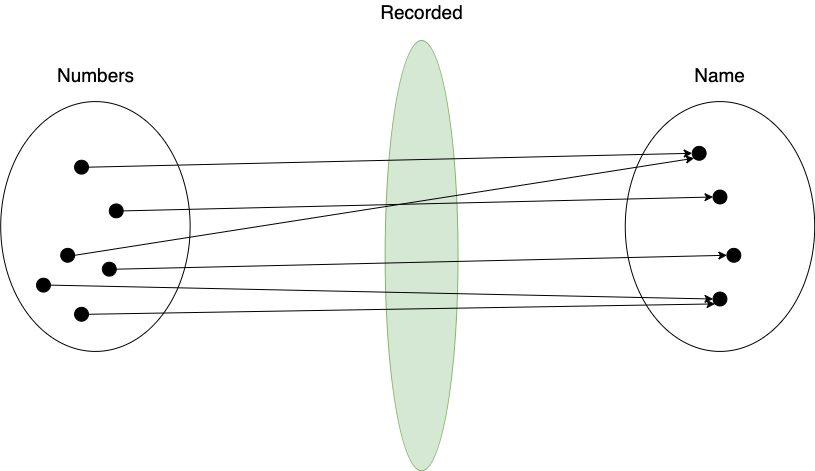
\includegraphics[scale=0.45]{images/Diagram.png}
    \caption{State of the System}
    \label{fig:Diagram}
    \end{figure}

% QUESTION 2 %
\item $numbers$ can be formally defined as: \\
$\{ \forall x, y: numbers | (x \in numbers \wedge y \in numbers) \rightarrow x \neq y \}$

% QUESTION 3 %
\item \emph{recorded} has to be a function since it is mapping 2 sets (\emph{numbers} and \emph{NameType}) and every member in \emph{numbers} has to be associated to exactly one name in \emph{NameType}. \\
A function requires 2 sets A and B present and there exists assignments from elements in A to elements in B.

% QUESTION 4 %
\item 
    \begin{itemize}
        \item Domain of \emph{recorded} is \emph{numbers} since it is the set contains elements that can be used as input to function \emph{recorded}.
        \item Codomain of \emph{recorded} is \emph{NameType} since it is a set of elements that can possibly be derived from function \emph{recorded}.
    \end{itemize}
 
% QUESTION 5 %
\item As previously stated, the domain of \emph{recorded} is \emph{numbers}. We know that \emph{numbers} is the set of all phone numbers recorded in contacts. Since not all elements of \emph{PhoneNumberType} are recorded, we can
state that \emph{numbers} is a subset of \emph{PhoneNumberType} as shown in the diagram displayed at \underline{question 1}.
A partial function \emph{f} is a function that is defined for some subset \emph{A'} of \emph{A}, not forcing mapping for 
all elements of set A such that $dom\text{  }f \subset A$. Thus, \emph{recorded} is a partial function.

% QUESTION 6 %
\item 
    \begin{itemize}
        \item Given the definition of an injective function ($\forall a, b | a \neq b \rightarrow f(a) \neq f(b) $), since multiple elements of \emph{numbers} can be associated with a single element of \emph{NameType}, then recorded is not injective. 
        \item Also, given the definition of a surjective function ($\forall b,   \exists a | f(a) = b$), since not all elements of \emph{NameType} are mapped to by at least one element of \emph{numbers}, \emph{recorded} is also not a surjective function. 

        \item Since it is neither injective nor surjective, recorded cannot be bijective. 
        \item[] $\rightarrow$ Therefore, \emph{recorded} is not one-to-one and not onto. 
    \end{itemize}

% QUESTION 7 %
\item The function \emph{recorded} can be formally defined as:\\
$\{ \exists y \in \emph{NameType},   \exists x \in \emph{numbers} | recorded(x) = y \}$

\end{enumerate}
